\subsection{The Turing machine $M_\text{binadd}$}

This Turing machine should recognize the language
\begin{align*}
    L_\text{binadd} = \{& w_1 \# w_2 \# w_3 \mid \text{$w_1$, $w_2$ and $w_3$ are binary numbers,} \\
    &\text{least significant bit first, and $w_1+w_2=w_3$} \}.
\end{align*}


\subsubsection{Description}

\paragraph{High-level description}
Move right along the tape, remembering the first $0$ or $1$ in the first two words, and replacing them with $X$. Then, compare the sum of these two symbols with the first number of the third number. Move back to the start and repeat this procedure until the first two numbers consist only of $X$s. If the third only consists of $X$s followed by $0$s (i.e. the tape looks like $X^*\#X^*\#X^*0^*$), accept.

If the fist two numbers are of different lengths, the shorter one is (for the purpose of the calculations) padded with $0$s after the the number itself. These $0$s should not be written to tape, but simply imagined. Refer to the implementation-level description for more information. 

\paragraph{Implementation-level description}
$M_{\text{binadd}}=$
``on input $w \in \{0,1,\#\}^*$:

\begin{enumerate}
    \item Remember\footnote{The term "remember" refers to creating as many states as necessary such that the different cell values follow different paths, but essentially, a specific path represents a specific value that was encountered.} the value $c=0$. This will represent the carry bit.
    \item \label{first_word_next_cell} Read the current cell and remember its value ($0$, $1$, or $\#$). We will call it $u$.
    \item If $u \neq \#$, write $X$ to the tape and sweep right until the next $\#$. This marks the end of the first word. 
    \item Sweep right until the current cell does not read $X$. Remember the contents of that cell (we will call it $v$).
    \item If $v \neq \#$, write $X$ to the tape and sweep right until the next $\#$. This marks the end of the second word.
    \item Sweep right until the current cell does not read $X$.
        \begin{itemize}
            \item
                If $u=v=\#$ and $c=0$, read until the end of the tape ($\_$).
                Accept if we encounter only $0$s until we reach the end of tape symbol.
                Reject otherwise.
            \item
                If $u=v=\#$ and $c=1$, read the current cell.
                Reject if it is not $1$. Accept if it is $\_$.
                Otherwise, read until the end of the tape ($\_$).
                Accept if we encounter only $0$s until we reach the end of tape symbol.
                Reject otherwise.
            \item
                Otherwise (i.e. if $u \neq \#$ or $v \neq \#$) read the value of the current cell, remember it as $t$, and replace its contents with $X$. To continue, consider the following table.
                \begin{center}
                    \begin{tabular}{cccc|c}
                        \multicolumn{4}{c|}{current value} & remember \\
                        $c$ & $u$ & $v$ & $t$ & $c$  \\
                        \hline
                        $0$ & $0,\#$ & $0,\#$ & $0$ & $0$ \\
                        $0$ & $0,\#$ & $1$ & $1$ & $0$ \\
                        $0$ & 1 & $0,\#$ & $1$ & $0$ \\
                        $0$ & $1$ & $1$ & $0$ & $1$ \\
                        $1$ & $0,\#$ & $0,\#$ & $1$ & $0$ \\
                        $1$ & $0,\#$ & $1$ & $0$ & $1$ \\
                        $1$ & 1 & $0,\#$ & $0$ & $1$ \\
                        $1$ & $1$ & $1$ & $1$ & $1$ \\
                    \end{tabular}
                \end{center}
                If the current set of values of $c,u,v,t$ is not represented in the table, reject. If it is, set $c$ to the respective value of the remember column and move on to the next step.
            \item Move left until we encounter $\#$. This marks the end of the second word. Move left until we encounter $\#$ again. This marks the end of the first word.
            \item Move left until we encounter $X$. Then move right one cell and go to step \ref{first_word_next_cell}."
        \end{itemize}
\end{enumerate}

\subsubsection{Theoretical analysis of complexity}

Let $f(n)$ denote the maximum number of steps for an input word of length $n$ again. 
The word that maximizes the number of steps required to reach a halting state for $n>2$ is $x_n=\# 0^{n-2} \#$. 
This is because the machine will have to cross the entirety of the middle word each time, marking off one letter at a time, until reaching the accepting state. 

\begin{wrapfigure}{r}{0.25\textwidth}
    \centering
    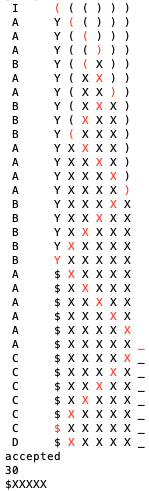
\includegraphics[width=2.5cm]{images/screenshots/paren.png}
    \vspace{-5cm}
\end{wrapfigure}

For these input words:

\begin{enumerate}
    \item We move right for $n$ steps to reach the end of the tape. While doing so, we marked off the next unmarked $0$ of the middle word. 
    \item We move left to the beginning of the tape ($n$ steps).
    \item We require two more transitions to return to the initial step ($2$ steps).
    \item We repeat steps 1-3 for a total of $n-2$ times because that is the length of the middle word (it will be marked off entirely).
    \item Finally, we need to move to the end of the tape to make sure there were no letters left in the final word ($n$ steps).
\end{enumerate}

The screenshot on the right shows an example for the input word $\#000\#$.

Steps 1 to 3 require a total of $2n+2$ transitions. These steps are carried out a total of $n-2$ times, so we have $(n-2)(2n+2)$ transitions. Finally, the last step requires $n$ transitions. We arrive at
\begin{align*}
    f_{n>2}(n)
    &= (n-2)(2n+2) + n \\
    &= 2n^2 - n - 4.
\end{align*}

Brute forcing the possible input words of length $0 \leq n \leq 2$, we find $f(0)=0$, $f(1)=1$, and $f(2)=2$. To obtain $f(n)$ for all $n$, we simply take $f_{n>2}+4$, yielding
$$ f(n) = 2n^2 - n. $$

As a result,
$$ M_\text{binadd} \in \text{DTIME}(2n^2-n), $$
and so its complexity is in the order of $\mathcal{O}(n^2)$.

\subsubsection{Paractical analysis of complexity}

The theoretical results are evident in practical trials. The data collected in \code{data/binadd-accepting\_zeros.csv} confirms the findings of $f$ (the values were cross-checked). Furthermore, the plot below shows how this worst-case scenario behaves as a plot of $n$ against the number of transitions made by the machine. 

\begin{center}
    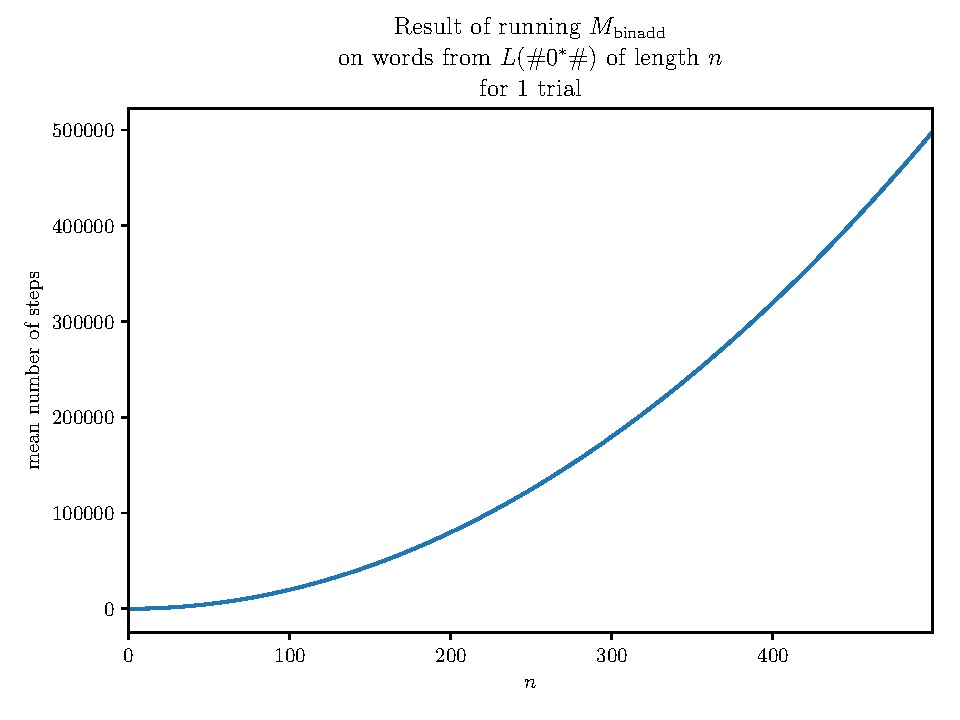
\includegraphics[width=\textwidth]{images/plots/binadd-accepting_zeros.pdf}
\end{center}

Other types of input words were also tested; please refer to the plots in section \ref{plots_binadd}, as well as the CSV data in \code{data/binadd-*.csv}. 